\documentclass[14pt]{extreport}
\usepackage{cmap}
\usepackage[utf8]{inputenc}
\usepackage[english,ukrainian]{babel}
\usepackage{graphicx}
\usepackage{geometry}
\usepackage{listings}
\usepackage{amsmath}
\usepackage{float}
\geometry{
	a4paper,
	left=20mm,
	right=20mm,
	top=20mm,
	bottom=20mm
}
\lstset{
	language=bash,
	tabsize=4,
	breaklines,
	keepspaces,
	showstringspaces=false,
}
\graphicspath{ {./pictures} }
\setlength{\parindent}{4em}

\newcommand\subject{Кросплатформне програмування}
\newcommand\lecturer{доцент кафедри ПЗ\\Дяконюк Л.М.}
\newcommand\teacher{ст. викл. кафедри ПЗ\\Шкраб Р.Р.}
\newcommand\mygroup{ПЗ-32}
\newcommand\lab{7}
\newcommand\theme{Робота з потоками}
\newcommand\purpose{Навчитися працювати з потоками}

\begin{document}
\begin{normalsize}
	\begin{titlepage}
		\thispagestyle{empty}
		\begin{center}
			\textbf{МІНІСТЕРСТВО ОСВІТИ І НАУКИ УКРАЇНИ\\
				НАЦІОНАЛЬНИЙ УНІВЕРСИТЕТ "ЛЬВІВСЬКА ПОЛІТЕХНІКА"}
		\end{center}
		\begin{flushright}
			Інститут \textbf{КНІТ}\\
			Кафедра \textbf{ПЗ}
		\end{flushright}
		\vspace{160pt}
		\begin{center}
			\textbf{ЗВІТ}\\
			\vspace{10pt}
			До лабораторної роботи № \lab\\
			\textbf{На тему}: “\textit{\theme}”\\
			\textbf{З дисципліни}: “\subject”
		\end{center}
		\vspace{40pt}
		\begin{flushright}
			
			\textbf{Лектор}:\\
			\lecturer\\
			\vspace{10pt}
			\textbf{Виконав}:\\
			
			студент групи \mygroup\\
			Коваленко Д.М.\\
			\vspace{10pt}
			\textbf{Прийняв}:\\
			
			\teacher\\
			
			\vspace{28pt}
			«\rule{1cm}{0.15mm}» \rule{1.5cm}{0.15mm} 2023 р.\\
			$\sum$ = \rule{1cm}{0.15mm}……………\\
			
		\end{flushright}
		\vspace{\fill}
		\begin{center}
			\textbf{Львів — 2023}
		\end{center}
	\end{titlepage}
		
	\begin{description}
		\item[Тема.] \theme.
		\item[Мета.] \purpose.
	\end{description}
	

	\section*{Лабораторне завдання}
Створити класи для сутностей, описаних в завданні. Наповнити колекції даних
з текстових файлів. Для виконання завдань розробити меню. Для реалізації
використовувати технологію потоків Stream.API. Cеріалізувати колекції.	
	
	Створити класи для бібліотеки. Клас Книга повинен містити інформацію про
	автора, назву та рік видання.
	Клас Абонемент знатиме прізвище, ім’я та по-батькові, а також електронну
	адресу.
	Кожен читач може взяти певну кількість книг, список яких він зберігає.
	Адміністратор фіксує дату, коли читач забирає книгу і дату планового
	повернення, а також дату реального повернення.
	Клас бібліотека містить колекцію всіх книг та колекцію всіх абонементів, а
	також методи, які з цими колекціями можна здійснювати.
	
	Дано текст, який складається з багатьох стрічок. Речення можуть бути в кількох
	стрічках. Вважати, що відсутні перенесення слова.
	\begin{itemize}
\item Відсортувати всі книги за роком видання.
\item Створити список адресів для розсилки повідомлень для читачів, що взяли
більше ніж 2 книги.
\item Перевірити, скільки користувачів взяли книги заданого автора.
\item Знайти найбільшу кількість книг, взятого читачем бібліотеки.
\item Здійснити різну розсилку 2 групам користувачів. У першу групу занести
користувачів, які мають менше 2 книг. Їм повідомити про новинки бібліотеки. У
другу групу занести інших користувачів. Їм повідомити про вчасність повернення
книг.
\item  Створити список боржників на біжучу дату. Для кожного боржника вказати
список книг, які підлягають поверненню, з вказівкою кількості днів порушення
терміну.
	\end{itemize}
	\section*{Хід роботи}

	\textbf{\textit{Main.java}}
	\begin{lstlisting}
package com.example.lab7;

import javafx.application.Application;
import javafx.scene.Scene;
import javafx.scene.layout.VBox;
import javafx.stage.Stage;

public class Main extends Application {
	
	@Override
	public void start(Stage primaryStage) {
		primaryStage.setTitle("Thread Bank Simulation");
		
		// Create the main layout
		VBox root = new VBox();
		root.getChildren().add(new BankSimulation());
		
		Scene scene = new Scene(root, 600, 400);
		primaryStage.setScene(scene);
		
		primaryStage.show();
	}
	
	public static void main(String[] args) {
		launch(args);
	}
}

package com.example.lab7;

import javafx.geometry.Pos;
import javafx.scene.control.Button;
import javafx.scene.control.Label;
import javafx.scene.control.TextField;
import javafx.scene.layout.HBox;
import javafx.scene.layout.VBox;

public class BankSimulation extends VBox {
	
	public BankSimulation() {
		setupUI();
	}
	
	private void setupUI() {
		// Create UI elements
		TextField threadCountField = new TextField("5");
		TextField resourceLimitField = new TextField("1000");
		Button startButton = getStartButton(threadCountField, resourceLimitField);
		
		// Layout
		HBox inputBox = new HBox(10, new Label("Thread Count:"), threadCountField,
		new Label("Resource Limit:"), resourceLimitField, startButton);
		inputBox.setAlignment(Pos.CENTER);
		
		getChildren().addAll(inputBox, BankThreadPanel.getInstance());
	}
	
	private static Button getStartButton(TextField threadCountField, TextField resourceLimitField) {
		Button startButton = new Button("Start Simulation");
		
		// Event handler for the start button
		startButton.setOnAction(event -> {
			int threadCount = Integer.parseInt(threadCountField.getText());
			int resourceLimit = Integer.parseInt(resourceLimitField.getText());
			
			// Start the bank simulation
			Bank bank = new Bank(resourceLimit);
			for (int i = 0; i < threadCount; i++) {
				ClientThread clientThread = new ClientThread("Thread " + (i + 1), bank);
				clientThread.start();
			}
		});
		return startButton;
	}
}

	\end{lstlisting}	
	
	\begin{figure}[H]
		\centering
		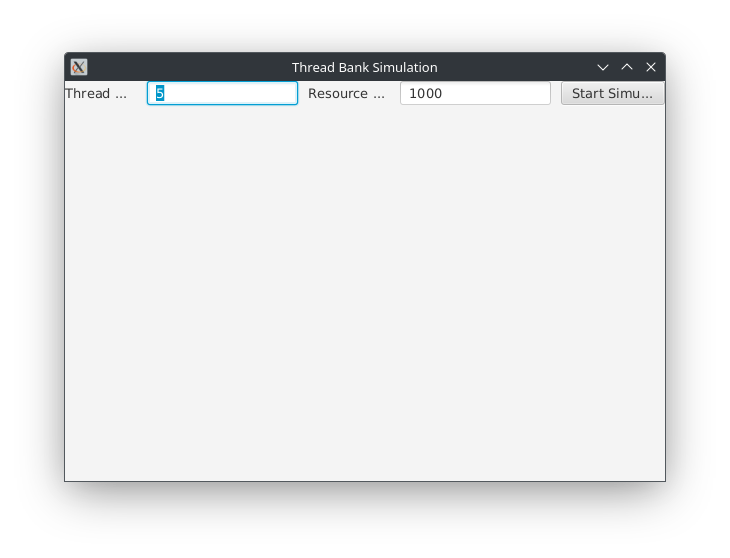
\includegraphics[scale=0.55]{1}
		\caption{Робота програми}
	\end{figure}

	\section*{Висновок}
	Під час виконання лабораторної роботи я працював з потоками. Навчився працювати з потоками.
	 
\end{normalsize}
\end{document}
